\documentclass[conference]{IEEEtran}
\usepackage{cite}
\usepackage{amsmath,amssymb,amsfonts}
\usepackage{algorithmic}
\usepackage{graphicx}
\usepackage{textcomp}
\usepackage{listings}
\newcommand{\missingNumber}{\textcolor{red}{XX}\xspace}
\newcommand{\missingPercentage}{\textcolor{red}{XX\%}\xspace}
\newcommand{\missingTable}{\textcolor{red}{XXTable}\xspace}
\newcommand{\missingGraph}{\textcolor{red}{XXGraph}\xspace}
\usepackage[usenames,dvipsnames]{xcolor} 
\usepackage{xspace} 

\graphicspath{{img/}}

\lstset{ 
	language=R,                     % the language of the code
	basicstyle=\ttfamily, % the size of the fonts that are used for the code
	numbers=left,                   % where to put the line-numbers
	numberstyle=\color{Blue},  % the style that is used for the line-numbers
	stepnumber=1,                   % the step between two line-numbers. If it is 1, each line
	% will be numbered
	numbersep=2pt,                  % how far the line-numbers are from the code
	backgroundcolor=\color{white},  % choose the background color. You must add \usepackage{color}
	showspaces=false,               % show spaces adding particular underscores
	showstringspaces=false,         % underline spaces within strings
	showtabs=false,                 % show tabs within strings adding particular underscores
	%frame=single,                   % adds a frame around the code
	rulecolor=\color{black},        % if not set, the frame-color may be changed on line-breaks within not-black text (e.g. commens (green here))
	tabsize=2,                      % sets default tabsize to 2 spaces
	captionpos=b,                   % sets the caption-position to bottom
	breaklines=true,                % sets automatic line breaking
	breakatwhitespace=false,        % sets if automatic breaks should only happen at whitespace
	keywordstyle=\color{RoyalBlue},      % keyword style
	commentstyle=\color{YellowGreen},   % comment style
	stringstyle=\color{ForestGreen}      % string literal style
} 
\begin{document}

\title{A Large-Scale Study of the Use of Eval in R}
\author{\vspace{-.8cm}\IEEEauthorblockN{
    \it\Large The Eval that Data Scientists Do}%
  %\IEEEauthorblockA{ dept} \\ \and
}  
\maketitle

\newcommand{\eval}{\texttt{eval}\xspace}
\renewcommand{\c}[1]{\lstinline{#1}\xspace}
\newcommand{\miss}[1]{{\textcolor{red}{#1}}\xspace}

\begin{abstract}
  The \eval function turns text into code. From the point of view of
  reasoning about software system, uses of \eval turn the program's code
  from a statically known quantity that can be reasoned about and analyzed
  into one of the inputs to the program. Thus, widespread use of \eval
  hinders our ability to provide safety and security guarantees for
  software. Understanding how \eval is used in practice is key to finding
  ways to mitigate its damage. One question that has not been studied is
  whether the usage of \eval is dependent on the application domain or other
  features of the language. This paper is a large-scale study of a corpus of
  \miss{3} million lines of data science libraries and end-user written in
  the R language. We performed a simple static analysis and more
  sophisticated dynamic analysis to confirm that \eval is indeed in wide
  spread use, and to categorized patters of usage. We found that \eval in
  this code base is more dangerous in some ways, and safer in others, than
  what was previously reported for JavaScript.
\end{abstract}

\section{Introduction}

Traditional program analysis techniques are based on sound reasoning about
program behavior, a program analyzer computes an over-approximation of the
set of possible operations performed by the system being
analyzed~\cite{cc77}.  This is predicated on knowing the program's code, and
computing that code's behavior for all possible inputs. The presence of
\eval entails that the program's input, any string variable, may be
reflected into its code giving rise to \emph{any} behavior allowed by the
language semantics. In many dynamic languages, \eval can redefine most
user-defined and built-in functions resulting in a complete loss of
precision for any operation following \eval. A group of influential
resaerchers argued to give up on soundness and, instead, to
under-approximate dynamic features~\cite{soundy} In their words ``a
practical analysis, therefore, may pretend that \eval does nothing, unless
it can precisely resolve its string argument at compile time.''  Assuming
that \eval does not have side-effects may be too optimistic. We rather
propose to study what \eval does in practice, in real-world code, so as to
give researchers data about how to better under-approximate uses of that
feature.

While there has been previous work investigating the usage of \eval in web
programming and JavaScript~\cite{ecoop11}, there are no other studies that
shed light on the usage of \eval in other programming languages and
application domains.  It is thus reasonable to wonder if the results from
previous work can be carried over to other contexts. For this paper, we have
picked the data science language R~\cite{r} as our object of study. R is
both different from JavaScript in linguistic terms and in terms of its user
base. JavaScript was designed to run untrusted code in browser, while R was
design for statistical computing on a desktop. JavaScript is used as a
general purpose language by a wide community of programmers; while R is used
for scientific computing by data scientist and domain experts with, often,
limited programming experience.

This paper sets out to highlight the differences in usage patterns of \eval
between these two languages and user communities. Our results are broadly
applicable as they increase our understanding of the range of uses of \eval,
present new use-cases, and, hopefully, provide insights into reasonable
under-approximations. More narrowly, for researchers interested in static
analysis of data science code, we provide a publicly available corpus of
programs and a toolchain that can be customized to deliver fine-grained
information about the usage and impact of \eval.

Our methodology for this work bows to the fact that static analysis of R is
difficult, instead we focus on dynamic analysis. To observe \eval we have
built a two-level monitoring infrastructure: we are able to monitor R
programs by instrumentation -- this gives us access to many user-visible
properties of R programs -- and we also can monitor the inner working of the
R interpreter -- this allows us to capture details of execution that are not
exposed at the source level.

Our corpus has been constructed to reflect the different level of
sophistication in the R community. We distinguish between the core
implementers of the language, developers with both extensive programming
experience and keen understanding of the language semantics, library
implementers, developers with some programming experience and a working
knowledge of R, and end-users, who are typically not expert programmers and
often have only a cursory knowledge of the language.\footnote{To illustrate
  the above consider that R uses lazy evaluation like Haskell. The authors
  have informally surveyed end-users, some of them computer scientists, and
  did not find a single one aware of that fact. Library developers, on the
  other hand, tend to know about laziness and program defensively around
  it.}  Thus, our corpus distinguished between \emph{core packages} (there
are \miss{8} such packages that are loaded together with the R virtual
machine), \emph{CRAN packages} (we selected \miss{500} curated packages that
pass stringent community quality checks and are equipped with tests and
sample data), \emph{scripts} (we used \miss{400} end-user written programs
that performs a particular data analysis task).  There are reasons to
believe that \eval usage patterns may differ between these datasets. The
core R code is extremely stable, it has only been maintained for the last 20
years with very few far reaching changes. The libraries represent a more
lively ecosystem with new libraries added each day.  Finally, end user code
is often one-use scripts thrown together and sometimes never revisited.


To understand the behavior of eval we perform a combination of static
analysis, dynamic analysis and manual inspection. The results presented
here summarize our findings.

Our infrastructure is publicly available, released in open source, and our
data, and code will be submitted to artifact evaluation.


\section{Related Work}

\cite{ecoop11}

Previous work looked at eval in JavaScript

Othere languages

Dynamic analysis


\section{Shades of Eval}

- Talk about environments
- How is it different from JS (takes language, env in R but string in JS).

\section{The Design of Eval}

There are four different kinds of \eval in the \emph{base} package:  \c{eval}, \c{evalq}, \c{eval.parent},  \c{local}.
The most important one is \eval: 

\begin{lstlisting}
eval <- function (expr, envir = parent.frame(), enclos = if (is.list(envir) || is.pairlist(envir)) parent.frame() else baseenv())  
	.Internal(eval(expr, envir, enclos))
\end{lstlisting}




The three other functions are defined using \lstinline|eval|.

\begin{lstlisting}
evalq <- function (expr, envir = parent.frame(), enclos = if (is.list(envir) || is.pairlist(envir)) parent.frame() else baseenv())  
	.Internal(eval(substitute(expr), envir, enclos))
	
eval.parent <- function (expr, n = 1) 
{
	p <- parent.frame(n + 1)
	eval(expr, p)
}

local <- function (expr, envir = new.env()) eval.parent(substitute(eval(quote(expr), envir)))
\end{lstlisting}


\c{expr} is the expression to be evaluated. It is not a string as in javascript. In order to evaluate a string, it should be first parsed using \c(parse(text = str)) to get an expression.

\eval makes it possible to specify the environment in which to evaluate the expression. \c{enclos} is an additional environment used for lookup when \c{envir} is a list, a pairlist or a dataframe. In that case, \c{envir} is copied into a temporary environment enclosed in \c{enclos}.

The \c{expr} argument of \eval is first evaluated in the current scope, then passed to the \eval. Quoting that argument prevents if from being evaluated in the current environment. \c{evalq} is a shortcut for \c{eval(quote(expr), ...)}. In the following code snippet, variable \c{r} is first looked up in the current scope with \eval whereas it is looked up in \c{env} with \c{evalq}.

\begin{lstlisting}
> r <- 5
> env <- new.env()
> env$r <- 9
> eval(r, env)
[1] 5
> evalq(r, envir = env)
[1] 9
\end{lstlisting}

\eval will return unchanged basic types such as vectors, functions, strings and environments. Promises are forced by \eval. Symbols are looked up in the current environment. Calls and expressions are evaluated. 

\section{Infrastructure}


\section{Corpus of R Programs}


\section{Threats to Validity}


\section{Research Question}
This section presents the results of our empirical study of eval in the R language.
\subsection{How many evals}

In our corpus eval is called \missingNumber times out of \missingNumber
total calls to all R functions. This is merely \missingPercentage of the total
number of calls. \missingTable breaks down the number of calls and callsites for
the four kinds of eval functions from the three source; core R, packages and
Kaggle code.

The core R packages are the biggest consumers of eval. Majority of calls,
\missingPercentage, originate from the core R packages. Kaggle code, which is
end-user code, has merely \missingNumber calls to eval.

Of the \missingNumber packages in our corpus, only \missingNumber packages call
eval. \missingTable shows the number of calls to eval made by the ten most
frequent callers to eval. \missingNumber packages account for over
\missingPercentage calls to eval.

\missingGraph shows the distribution of number of callsites to eval across these
packages. \missingNumber packages have a single eval callsite.


\subsection{How are they used}

- classify evals based on what they can be replaced with

\subsubsection{A taxonomy of \c{eval}}

We first classify \c{eval} depending on the resolved expression, \emph{i.e.}
the first argument of \c{eval} after all possible function calls and symbol
resolution in it have been executed.




\subsection{How to replace evals}

We look at how \emph{polymorphic} the \c{expr} argument of \eval can be, \emph{i.e.} how many different types of the resolved \c{expr} there are per call sites, in Figure~\ref{fig:polymorphism}. 89\% of the call sites are \emph{monomorphic}.

\begin{figure}
    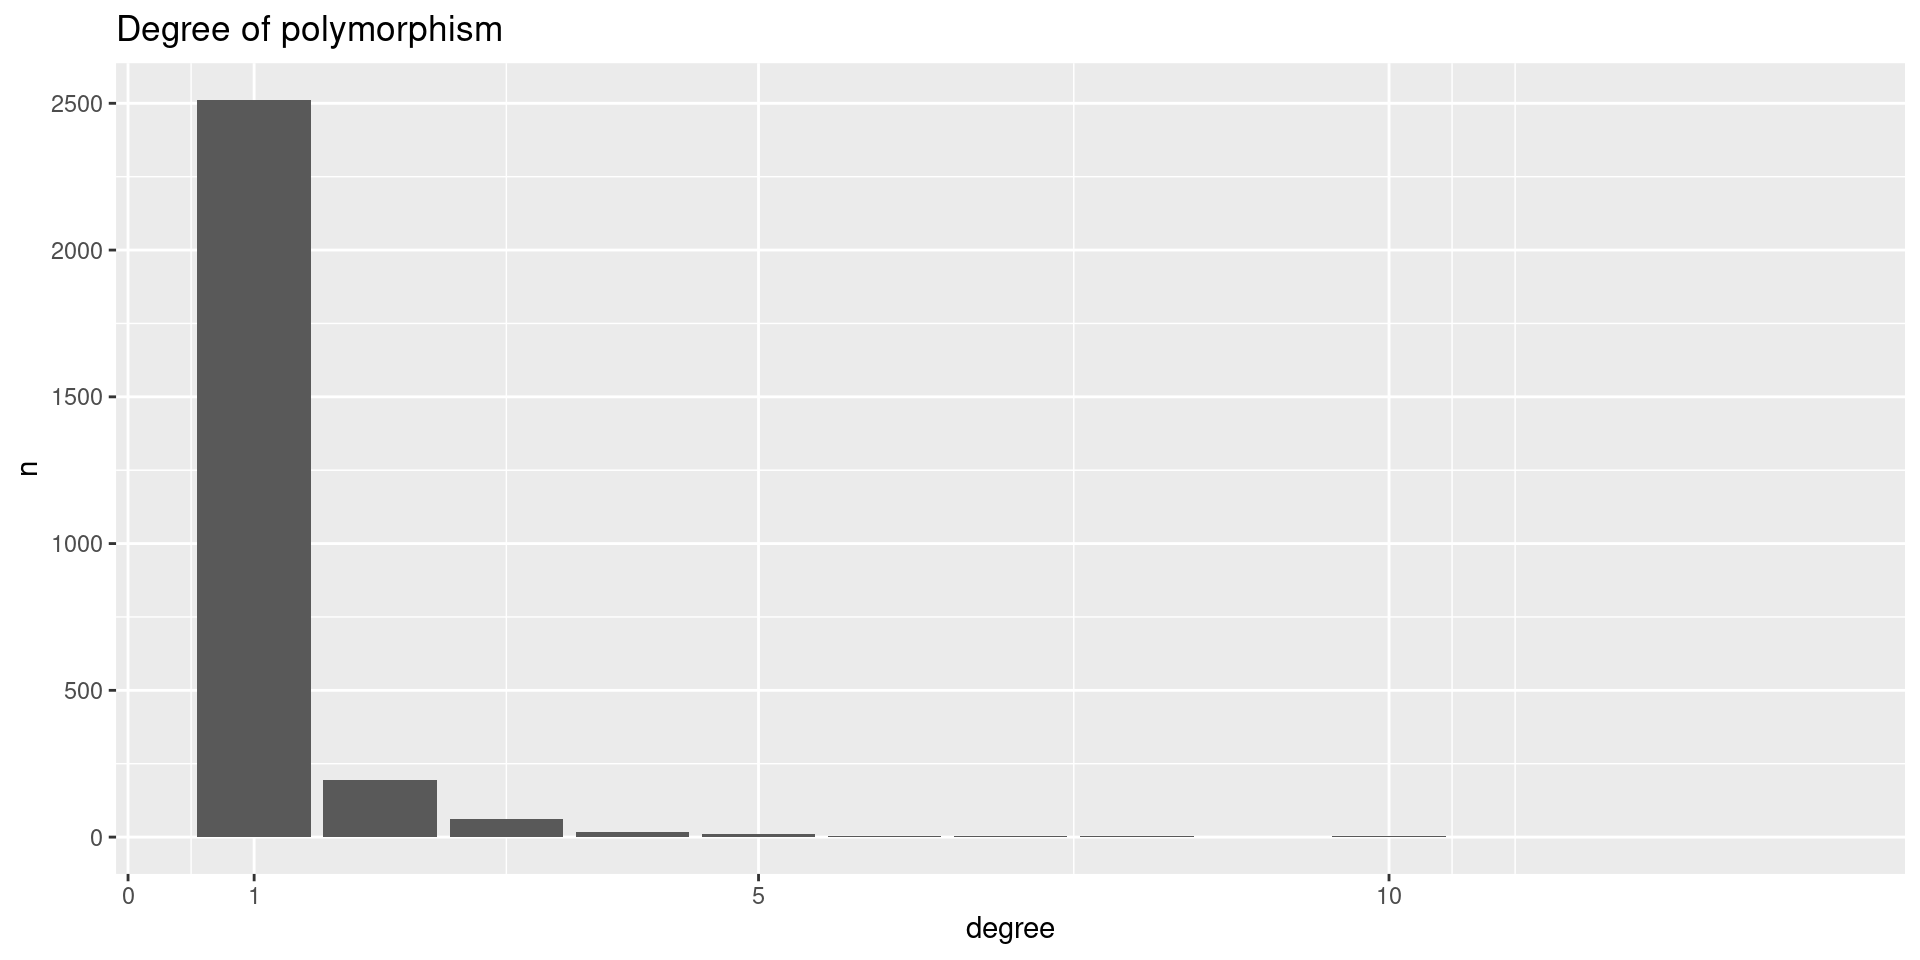
\includegraphics[width=\columnwidth]{polymorphism-1}
    \caption{Degree of polymorphism of \c{expr} per call sites.} \label{fig:polymorphism}
\end{figure}

\subsection{How dangerous is eval}

\subsection{How many evals can be replaced}

\section{Case studies}

\subsection{base}


\section{Conclusion}

\bibliographystyle{IEEEtran}
\bibliography{bib/bibliography,bib/jv}

\end{document}


Eval is evil, we would like to replace it.
Research Questions
How often is eval used? 
How often it is used in base / other packages?
blocking: cannot find out precisely what comes from base
What is the source of evals?
Provenance (source arguments to eval)
How many evals are in libraries / vignettes
What is eval used for?
??Eval in the tidyverse
TODO: Classification of evals in  packages (Pierre)
TODO: look at the first function to get
binary / unary / assignment / other function
does it have {
evals that do nothing (they get values)
...
TODO: In the case of base package (Filip)
access default values of formals
simply implementation
weird replacement of calls (write.csv -> write.table)
accessing variable from another environment (instead of get)
evaling user input
Change of caller pattern: 
m <- match.call()
 m$name <- NULL
 m[[1L]] <- as.name("library")
eval(m, .GlobalEnv)
     - 	TODO: How dangerous is eval? (Aviral)
Does eval generate new code (create new functions)?
environment writes (reads)
system environment variables
connections
random number generator - setting seed
Does eval do dynamic code loading?
Does eval argument reflect on the call stack?
Calls to C Code
TODO: Could the eval be made safer?
TODO: Could some of the eval calls be replaced?
